\documentclass{beamer}
\usetheme{metropolis}

\usepackage[ngerman]{babel}
\usepackage[autostyle=true,german=quotes]{csquotes}
\usepackage[linewidth=1pt]{mdframed}
\usepackage{hyperref}
\usepackage{makecell}
\usepackage{pifont}
\usepackage{tikz}
\usetikzlibrary{positioning, calc, arrows, fit, decorations.pathreplacing, shapes, shapes.multipart, snakes}
\usepackage{verbatim}
\usepackage{tabularx}
\usepackage{textcomp}
\usepackage{centernot}
\usepackage{amsmath}
\usepackage{xcolor}
\usepackage{tikz}
\usepackage{underscore}

\batchmode

\hypersetup{
	colorlinks,
	urlcolor=blue,
	linkcolor=black % for ToC
}
\newenvironment{qaa}[1]{
	#1

	\begin{mdframed}
		\small
}{
	\end{mdframed}
}

\newcommand{\true}{\ding{51}}
\newcommand{\false}{\ding{55}}
\newcommand{\code}[1]{
	\begin{mdframed}
		\verbatiminput{#1}
	\end{mdframed}
}

\title{Tutorium 14: Compiler}
% \subtitle{}
\author{Paul Brinkmeier}
\institute{Tutorium Programmierparadigmen am KIT}
\date{04. Februar 2020}

\begin{document}

\begin{frame}
	\titlepage
\end{frame}

\section{Einführung}

\begin{frame}{Compiler in ProPa}
	\begin{itemize}
		\item Ein bisschen...
		\begin{itemize}
			\item Lexikalische Analyse (Tokenisierung)
			\item Syntaktische Analyse (Parsen)
			\item \textcolor{gray}{Semantische Analyse (Optimierung)}
			\item Codegenerierung
		\end{itemize}
		\pause
		\item Klausur:
		\begin{itemize}
			\item SLL(k)-Form beweisen
			\item Rekursiven Abstiegsparser schreiben/vervollständigen
			\item First/Follow-Mengen berechnen
			\item Java-Bytecode
				% Zeigen: Java-BC-Aufgabe (16SS), Code-Generierung nächste Mittwoch und Freitag (findet noch statt)
		\end{itemize}
	\end{itemize}
\end{frame}

\subsection{Syntaktische Analyse (18WS)}

\begin{frame}{Syntaktische Analyse (18WS)}
	\begin{align*}
		SGML \to & \;\; \textrm{\texttt{< id >}} \;\; Children \;\; \textrm{\texttt{< / >}}\\
		Children \to & \;\; \epsilon \mid SGML \;\; Children
	\end{align*}

	\begin{equation*}
		\{\textrm{\texttt{<id><id></><id></></>}},\;\;\textrm{\texttt{<id></>}},\;\;...\} \in G
	\end{equation*}

	\pause
	\begin{itemize}
		\item Begründen Sie formal, dass die obige Grammatik nicht in $\textrm{SLL}(1)$-Form ist (3P.).
		\pause
		\item Entwickeln Sie für [eine linksfaktorisierte Version der obigen Grammatik] einen rekursiven Abstiegsparser (16P.).
	\end{itemize}
\end{frame}

\begin{frame}{Java-Bytecode (16SS)}
	\footnotesize
	Übersetzen Sie folgenden Java-Programmausschnitt in Java-Bytecode (10P.):

	\code{code/bytecode16ss.java}

	\pause
	Hinweise:

	\begin{itemize}
		\item Codeerzeugung für bedingte Sprünge: Folien 447ff.
		\item Um eine Bedingung der Form \texttt{!cond} zu übersetzen, reicht es, \texttt{cond} zu übersetzen und die Sprungziele anzupassen.
	\end{itemize}
\end{frame}

% Aufgaben:
% Nicht-SLL(1)-Teilmenge von JSON-Subset ist SLL(n) für n \in 1, 2?
% Rekursiver Abstieg für JSON-Subset
% Rekursiver Abstieg für Klausuraufgabenliste
% Java Bytecode

\section{Compiler}

\subsection{Motivation}

\begin{frame}{Compiler: Motivation}
	\begin{itemize}
		\item Maschine(-nmodell) versteht i.d.R. eingeschränkten Instruktionssatz
		\begin{itemize}
			\item Es gibt/gab zwar auch mal CISC-Maschinen, heute ist sind aber RISC(-ähnliche) Prozessoren am weitesten verbreitet
			\item Gründe: RISC-Prozessoren sind wesentlich einfacher (= billiger) zu bauen
		\end{itemize}
		\item Programme in Maschinensprache sind i.d.R. für Menschen nicht einfach zu Schreiben.
		\pause
		\item Also: Erfinde einfacher zu Schreibende ($\approx$ mächtigere) Sprache, die dann in die Sprache der Maschine übersetzt wird.
		\item Diesen Übersetzungsschritt sollte optimalerweise ein Programm erledigen, da wir sonst auch einfach direkt Maschinensprache-Programme schreiben können.
	\end{itemize}
\end{frame}

\begin{frame}{Compiler}
	\begin{itemize}
		\item Übersetzer für formale Sprachen nennt man \emph{Compiler}
		\item Beispiele:
		\begin{itemize}
			\item C, Haskell, Rust, Go $\to$ X86
			\item Java, Clojure, Kotlin $\to$ Java-Bytecode
			\item TypeScript $\to$ JavaScript
			\item \textcolor{gray}{Python $\to$ Python-AST}
		\end{itemize}
		\pause
		\item \textcolor{gray}{Interpreter kann man auch als Compiler kategorisieren, sie zählen aber i.A. nicht dazu}
		\pause
		\item Single-pass vs. Multi-pass
		\begin{itemize}
			\item Single-pass: Eingabe wird einmal gelesen, Ausgabe währenddessen erzeugt (ältere Compiler)
			\item Multi-pass: Eingabe wird in Zwischenschritten in verschiedene Repräsentationen umgewandelt
			\begin{itemize}
				\item Quellsprache, Tokens, AST, Zwischensprache, Zielsprache
			\end{itemize}
		\end{itemize}
	\end{itemize}
\end{frame}

\subsection{Lexikalische Analyse}

\begin{frame}{Lexikalische Analyse}
	\begin{columns}
		\begin{column}{0.5\textwidth}
			\code{code/lexinput.java}
		\end{column}
		\begin{column}{0.5\textwidth}
			\code{code/lexoutput.java}
		\end{column}
	\end{columns}

	\begin{itemize}
		\item Lexikalische Analyse (Tokenisierung) verarbeitet eine Zeichensequenz in eine Liste von \emph{Tokens}.
		\item Tokens sind Zeichengruppen, denen eine Semantik innewohnt:
		\begin{itemize}
			\item \texttt{int} --- Typ einer Ganzzahl
			\item \texttt{=} --- Zuweisungsoperator
			\item \texttt{x1} --- Variablen- oder Methodenname
			\item \texttt{123} --- Literal einer Ganzzahl
			\item \texttt{"123"} --- String-Literal
			\item etc.
		\end{itemize}
		\item Lösbar mit regulären Ausdrücken, Automaten
	\end{itemize}
\end{frame}

\subsection{Syntaktische Analyse}

\begin{frame}{Syntaktische Analyse}
	\begin{itemize}
		\item Syntaktische Analyse stellt die unterliegende Struktur der bisher linear gelesenen Eingabe fest:
		\begin{itemize}
			\item Blockstruktur von Programmen
			\item Baumstruktur von HTML-Dateien
			\item Header, Inhalt-Struktur von Mails
			\item Verschachtelte mathematische Ausdrücke
		\end{itemize}
		\item Syntaktische Analyse ist das größte Compiler-Thema in PP.
		\pause
		\item Übliche Vorgehensweise (in PP):
		\begin{itemize}
			\item Grammatik $G$ erfinden
			\item ggf. $G$ in einfache Form $G'$ bringen
			\item rekursiven Abstiegsparser für $G'$ implementieren
		\end{itemize}
		\item Alternativ: Parser-Kombinatoren, Yacc, etc.
	\end{itemize}
\end{frame}

\begin{frame}{Beispiel: Mathematische Ausdrücke}
	\begin{columns}
		\begin{column}{0.5\textwidth}
			\begin{equation*}
				1 + 5 * 7 + 6
			\end{equation*}
		\end{column}
		\begin{column}{0.5\textwidth}
			\begin{figure}
				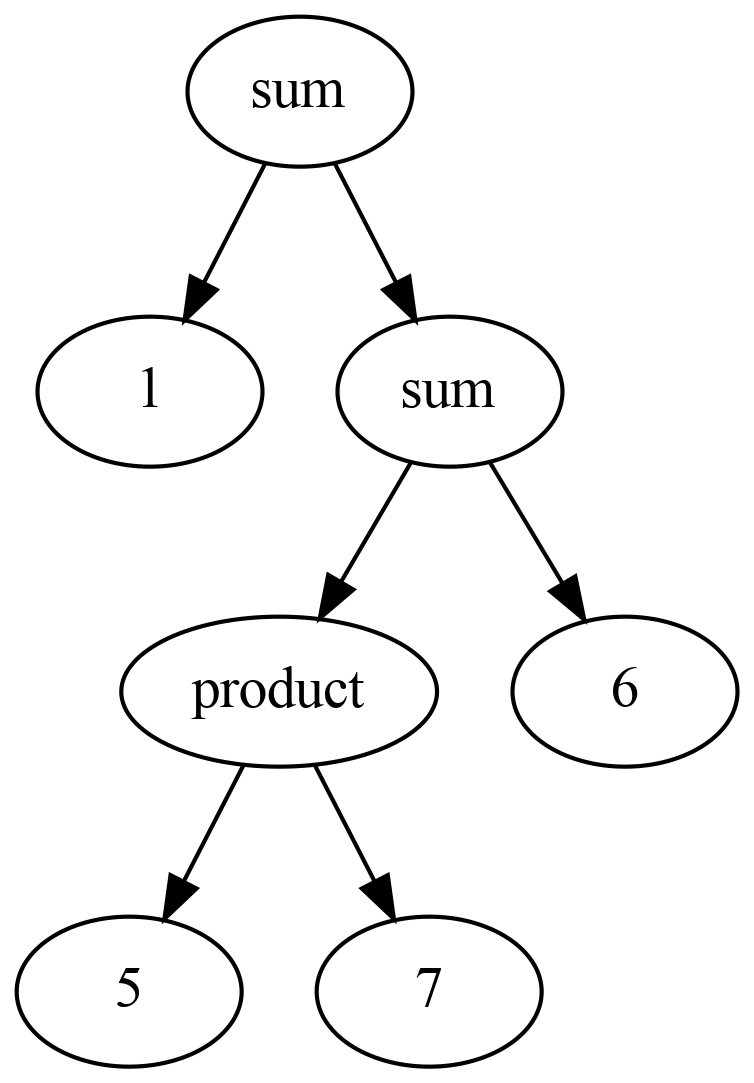
\includegraphics[width=0.65\textwidth]{images/baumstruktur.png}
			\end{figure}
		\end{column}
	\end{columns}

	\begin{itemize}
		\item Zu beachten: Punkt-vor-Strich (Präzedenz), Klammerung, etc.
		\item Nicht mehr mit regulären Ausdrücken lösbar
		\item \enquote{Offensichtliche} Grammatik oft nicht einfach zu Parsen
	\end{itemize}
\end{frame}

\begin{frame}{Beispiel: Mathematische Ausdrücke}
	\begin{equation*}
		E \to \;\; \textrm{\texttt{num}} \mid \textrm{\texttt{(}} \;\; E \;\; \textrm{\texttt{)}}
		 \mid E \;\; \textrm{\texttt{+}} \;\; E
		 \mid E \;\; \textrm{\texttt{*}} \;\; E
	\end{equation*}

	\pause

	\begin{columns}
		\begin{column}{0.5\textwidth}
			\begin{figure}
				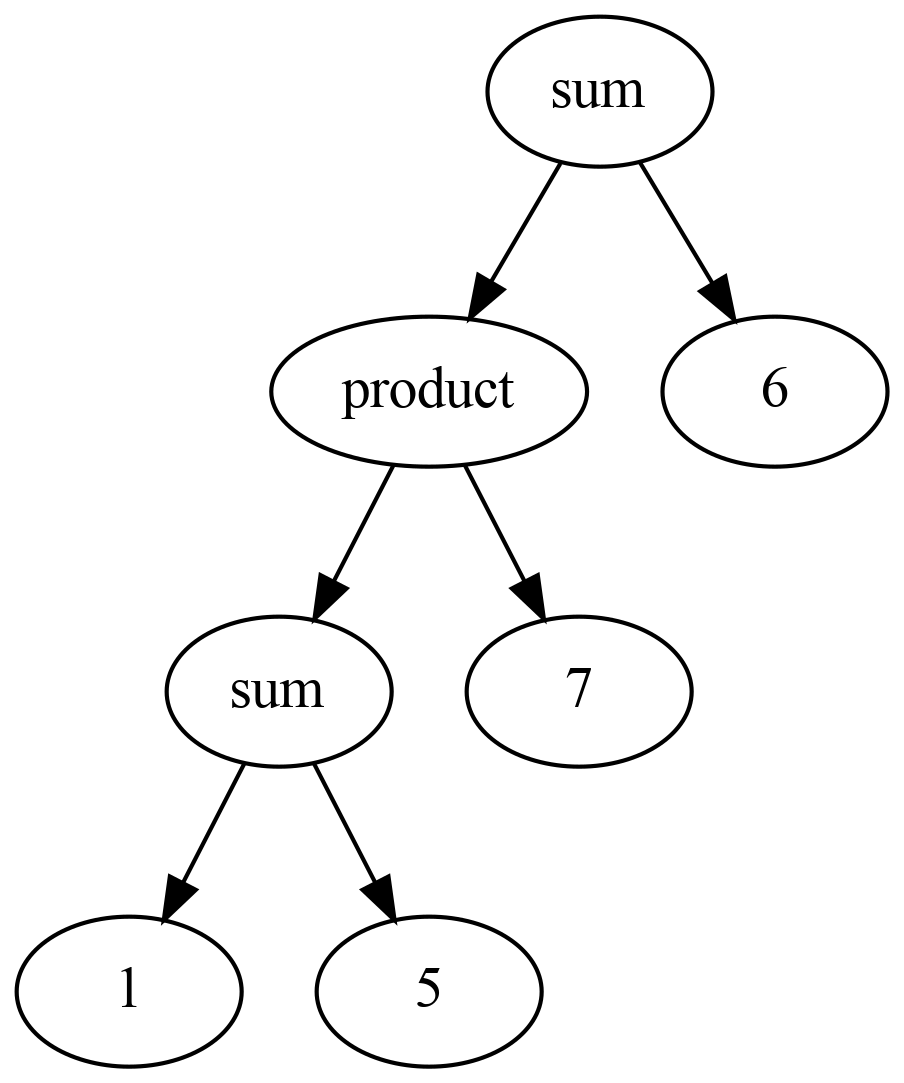
\includegraphics[width=0.65\textwidth]{images/baumstruktur2.png}
			\end{figure}
		\end{column}
		\begin{column}{0.5\textwidth}
			\begin{figure}
				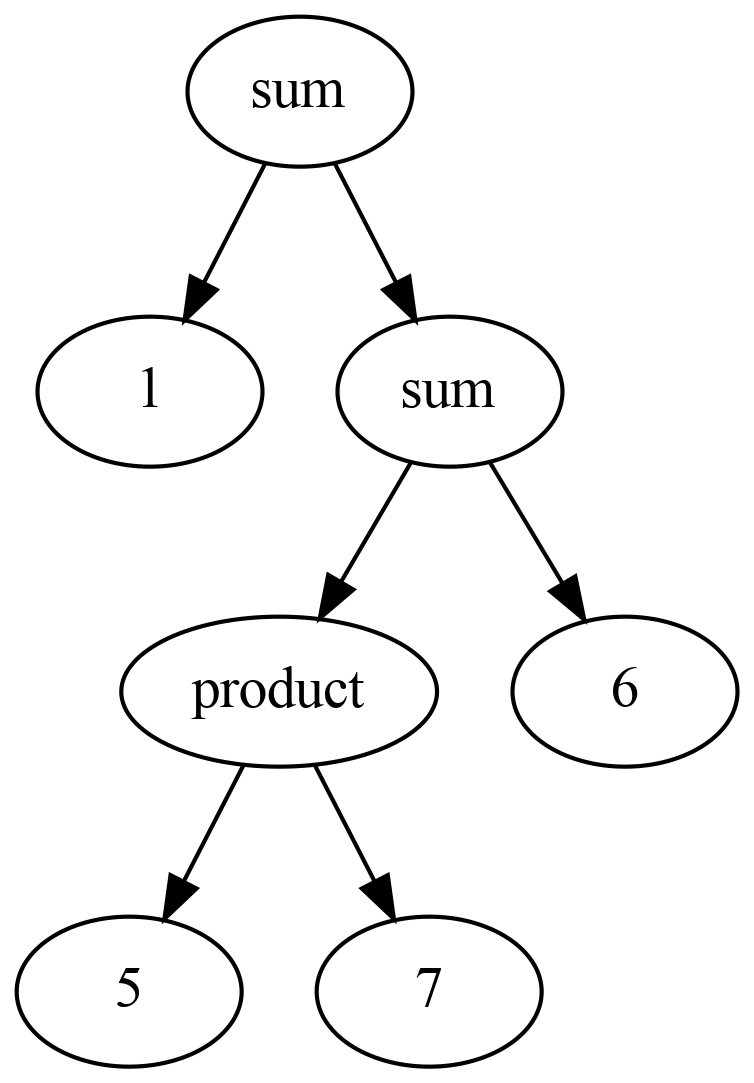
\includegraphics[width=0.65\textwidth]{images/baumstruktur.png}
			\end{figure}
		\end{column}
	\end{columns}

	\pause

	\begin{itemize}
		\item Ableitungsbaum nicht eindeutig $\leadsto$ schlecht
		\item Ableitungsbaum garantiert nicht Punkt-vor-Strich $\leadsto$ schlecht
	\end{itemize}
\end{frame}

\begin{frame}{Präzedenz, Linksfaktorisierung}
	Wie zeichnen sich \enquote{gute} Grammatiken aus?
	\pause

	Operatorpräzedenz schon in Grammatik definiert:
	\begin{align*}
		E \to & \;\; E \;\; \textrm{\texttt{+}} \;\; T \mid E \;\; \textrm{\texttt{-}} \;\; T \mid T\\
		T \to & \;\; T \;\; \textrm{\texttt{*}} \;\; F \mid T \;\; \textrm{\texttt{/}} \;\; F \mid F\\
		F \to & \;\; \textrm{\texttt{num}} \; | \; \textrm{\texttt{(}} \;\; E \;\; \textrm{\texttt{)}}
	\end{align*}

	\pause

	Vermeidung von Linksrekursion (Linksfaktorisierung):
	\begin{align*}
		E     \to & \;\; T \;\; EList\\
		EList \to & \;\; \epsilon \mid \textrm{\texttt{+}} \;\; T \;\; EList \mid \textrm{\texttt{-}} \;\; T \;\; EList\\
		T     \to & \;\; F \;\; TList\\
		TList \to & \;\; \epsilon \mid \textrm{\texttt{*}} \;\; F \;\; TList \mid \textrm{\texttt{/}} \;\; F \;\; TList\\
		F \to & \;\; \textrm{\texttt{num}} \; | \; \textrm{\texttt{(}} \;\; E \;\; \textrm{\texttt{)}}
	\end{align*}
\end{frame}

\begin{frame}{First-/Followmenge, Indizmenge}
	\footnotesize

	\begin{align*}
		EList \to & \;\; \epsilon \mid \textrm{\texttt{+}} \;\; T \;\; EList \mid \textrm{\texttt{-}} \;\; T \;\; EList
	\end{align*}
	
	Wie können wir bspw. bei $EList$ entscheiden, welche Produktion anzuwenden ist?
	\pause
	\begin{itemize}
		\item $\leadsto$ definiere \emph{Indizmenge} $IM_k(A \to \alpha) = \textrm{First}_k(\alpha \textrm{Follow}_k(A))$
		\item Wenn nächste $k$ Token in $IM_k(EList \to \phi)$ $\leadsto$ weiter mit $\phi$
		\pause
		\item $IM_1(EList \to \; \epsilon) = \textrm{First}_1(\epsilon \textrm{Follow}_1(EList)) = \{ \textrm{\texttt{)}}, \textrm{\texttt{\#}} \}$
		\item $IM_1(EList \to \; \textrm{\texttt{+}} \;\; T \;\; EList) = \textrm{First}_1(\textrm{\texttt{+}} \; T \; EList \; \textrm{Follow}_1(EList)) = \{ \textrm{\texttt{+}} \}$
		\item $IM_1(EList \to \; \textrm{\texttt{-}} \;\; T \;\; EList) = \textrm{First}_1(\textrm{\texttt{-}} \; T \; EList \; \textrm{Follow}_1(EList)) = \{ \textrm{\texttt{-}} \}$
		\pause
		\item $\textrm{First}_k(A)$: Menge an möglichen ersten $k$ Token in $A$
		\item $\textrm{Follow}_k(A)$: Menge an möglichen ersten $k$ Token nach $A$
	\end{itemize}
\end{frame}

\begin{frame}{SLL-Kriterium}
	Grammatik ist in $\textrm{SLL}(k)$-Form\\
	$:\Leftrightarrow \forall A \to \alpha, A \to \beta \in P: IM_k(A \to \alpha) \cap IM_k(A \to \beta) \neq \emptyset$

	\begin{itemize}
		\item $\textrm{SLL}(k)$: Bei einem Nichtterminal muss die zu wählende Produktion an den nächsten $k$ Token wählbar sein.
		\item Nichtterminale mit nur einer Produktion sind hier irrelevant
		\item Schwierig daran: $\textrm{Follow}$-Mengen berechnen
	\end{itemize}
	\pause
	\begin{align*}
		E \to & \;\; E \;\; \textrm{\texttt{+}} \;\; T \mid E \;\; \textrm{\texttt{-}} \;\; T \mid T\\
		T \to & \;\; T \;\; \textrm{\texttt{*}} \;\; F \mid T \;\; \textrm{\texttt{/}} \;\; F \mid F\\
		F \to & \;\; \textrm{\texttt{num}} \; | \; \textrm{\texttt{(}} \;\; E \;\; \textrm{\texttt{)}}
	\end{align*}
	
	\begin{itemize}
		\item Begründet formal, dass obige Grammatik nicht $\textrm{SLL}(1)$.
		\item Berechnet $\textrm{Follow}_1(N)$ für $N \in \{ E, T, F \}$.
	\end{itemize}
\end{frame}

\begin{frame}{Rekursive Abstiegsparser}
	\footnotesize
	\begin{align*}
		E     \to & \;\; T \;\; EList\\
		EList \to & \;\; \epsilon \mid \textrm{\texttt{+}} \;\; T \;\; EList \mid \textrm{\texttt{-}} \;\; T \;\; EList\\
		T     \to & \;\; F \;\; TList\\
		TList \to & \;\; \epsilon \mid \textrm{\texttt{*}} \;\; F \;\; TList \mid \textrm{\texttt{/}} \;\; F \;\; TList\\
		F \to & \;\; \textrm{\texttt{num}} \; | \; \textrm{\texttt{(}} \;\; E \;\; \textrm{\texttt{)}}
	\end{align*}
	\begin{itemize}
		\item Yay, unsere Grammatik hat jetzt $\textrm{SLL}(1)$-Form!
		\item Aber was bringt das?
		\pause
		\item $G$ ist jetzt einfach ausprogrammierbar:
		\begin{itemize}
			\item 1 Methode per Nichtterminal: \texttt{parseE()}, \texttt{parseEList()}, ...
			\item \texttt{Token[k]}-Instanzattribut für $k$ langen Lookahead
			\item \texttt{expect(TokenType)}-Methode, um Token zu verarbeiten
		\end{itemize}
		\pause
		\item Vervollständigt \texttt{demos/java/exprparser/ExprParser.java}!
	\end{itemize}
\end{frame}

\subsection{Semantische Analyse}

\begin{frame}{Semantische Analyse}
	\begin{itemize}
		\item PP beschäftigt sich (bis auf Typinferenz) nur kurz mit semantischer Analyse
		\item Hier geht es um Optimierungen, Typchecks, etc.
		\item $\leadsto$ weiterführende (Master-)Vorlesungen am IPD
	\end{itemize}
\end{frame}

\subsection{Codegenerierung}

\begin{frame}{Codegenerierung}
	\begin{figure}
		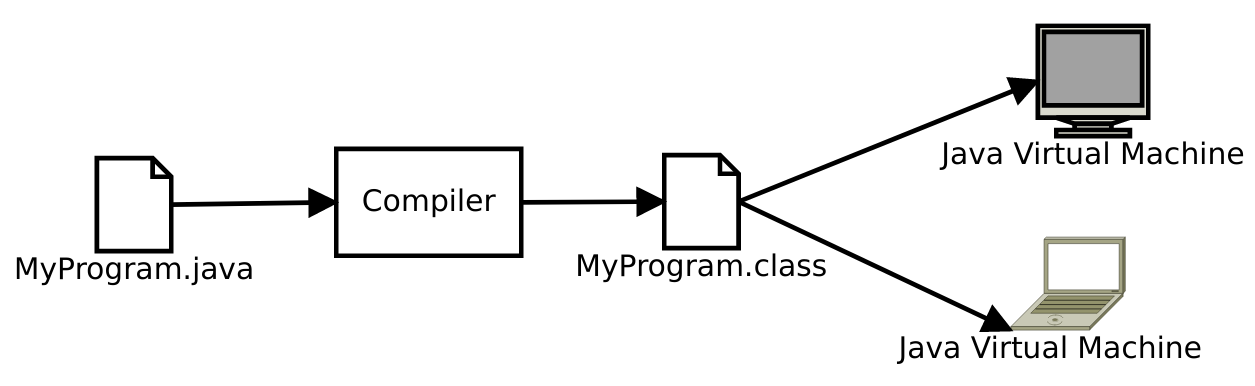
\includegraphics[width=\textwidth]{images/javabytecode}
	\end{figure}

	\begin{itemize}
		\item Codegenerierung wird in PP am Beispiel Java-Bytecode demonstriert
		\begin{itemize}
			\item \enquote{Jede_r kann Java}
			\item Relativ übersichtliche \enquote{Maschinensprache}
			\item Ggf. relevant, wenn seltsame Bugs in Java-Programmen auftreten
		\end{itemize}
	\end{itemize}
\end{frame}

\begin{frame}{Java-Bytecode: Lokale Variablen, Operandenstack}
	\begin{itemize}
		\item \texttt{?load_<x>}, \texttt{?store_<x>}
		\begin{itemize}
			\item \texttt{<x>}: ID einer lokalen Variablen
		\end{itemize}
		\item \texttt{?add}
		\item \texttt{?sub}
		\item \texttt{?mul}
		\item \texttt{bipush <c>}
		\item \texttt{?const_<c>}
	\end{itemize}

	\scriptsize

	\texttt{?}-Instruktionen gibt es für verschiedene Typen, bspw. \texttt{iadd}, \texttt{fadd}
\end{frame}

\begin{frame}{Java-Bytecode: Klassen, Methoden}
	\begin{itemize}
		\item \texttt{getfield <field>}, \texttt{putfield <field>}
		\item \texttt{invokevirtual <m>}, \texttt{invokestatic <m>}
		\item \texttt{new <t>}, \texttt{newarray <t>}
		\item \texttt{?return}
		\begin{itemize}
			\item \texttt{areturn} für Objekte
		\end{itemize}
	\end{itemize}
\end{frame}

\begin{frame}{Java-Bytecode: Sprünge}
	\begin{itemize}
		\item \texttt{goto <label>}
		\item \texttt{if(eq|ne|lt|gt|le|ge) <label>}
		\item \texttt{if_?cmp(eq|ne|lt|gt|le|ge) <label>}
	\end{itemize}
\end{frame}

\begin{frame}{Java-Bytecode: Codegenerierung}
	Kennen sollte man:

	\begin{itemize}
		\item Methodenaufrufe (\texttt{invokevirtual})
		\item Zugriff auf Attribute (\texttt{getfield}, \texttt{putfield})
		\item \texttt{if}, \texttt{while}
		\item Kurzauswertung (Laziness bei \texttt{\&\&} und \texttt{\string|\string|})
		\item Negation (Kein \texttt{not}-Befehl, nur veränderte Sprungziele)
	\end{itemize}
\end{frame}

\section{Ende}

\begin{frame}{Ende}
	\begin{itemize}
		\item Danke für's Kommen!
		\item Bei Fragen: \texttt{paul.brinkmeier@fsmi.uni-karlsruhe.de}
		\item Fragestunde mit den Übungsleitern:
		\begin{itemize}
			\item 16.03.2020, 14:00, Raum -101
		\end{itemize}
		\item \texttt{Klausuraufgaben.md} enthält jetzt auch die neuesten Klausuren
	\end{itemize}
\end{frame}

\end{document}
